\documentclass{article}

    % Input language encoding
    \usepackage[utf8]{inputenc}
   
    % Output languages
    \usepackage[english, greek]{babel}
    \usepackage{alphabeta}
    
    % Fonts
    \usepackage[T1,LGR]{fontenc}
    \usepackage{lmodern}

    % Special quotes - Recommended for biblatex
    \usepackage{csquotes}

    % Images
    \usepackage{graphicx}
    \usepackage{float}
    \usepackage{caption}
    \usepackage{subcaption}

    % Math
    \usepackage{amsmath}
    \usepackage{amssymb}

    % Paragraph Formatting
    \usepackage{parskip}

    % Code
    \usepackage{listings}
    \usepackage{fancyvrb}

    % Different Enumerations
    \usepackage{enumitem}

    % Trees
    \usepackage{qtree}

    % Other Drawings
    \usepackage{tikz}
    \usetikzlibrary{shapes,backgrounds}

    % Links
    \usepackage{hyperref}

    % Bibliography
    \usepackage[style=numeric]{biblatex}
    
    % Color
    \usepackage{color}
   
    % Setup

    % For hyperlinks
    \hypersetup{
        colorlinks=true,
        linkcolor=blue,
        filecolor=magenta,      
        urlcolor=cyan,
    }

    \urlstyle{same}
    
    % For code
    \definecolor{codegreen}{rgb}{0,0.6,0}
    \definecolor{codegray}{rgb}{0.5,0.5,0.5}
    \definecolor{codepurple}{rgb}{0.58,0,0.82}
    \definecolor{backcolour}{rgb}{0.95,0.95,0.92}
     
    \lstdefinestyle{mystyle}{
        backgroundcolor=\color{backcolour},   
        commentstyle=\color{codegreen},
        keywordstyle=\color{magenta},
        numberstyle=\tiny\color{codegray},
        stringstyle=\color{codepurple},
        basicstyle=\fontsize{8}{11}\selectfont\ttfamily,
        breakatwhitespace=false,         
        breaklines=true,                 
        captionpos=b,                    
        keepspaces=true,                 
        numbers=left,                    
        numbersep=5pt,                  
        showspaces=false,                
        showstringspaces=false,
        showtabs=false,                  
        tabsize=4
    }

    \lstset{style=mystyle}


    % For math
    \DeclareMathSizes{10}{10}{10}{10}
    \setlength{\parindent}{0cm}

    % Foreign Language macro
    \newcommand{\english}[1]{\foreignlanguage{english}{{#1}}}

    % Location of bibliography
    \addbibresource{bibliography.bib}

    % Location of images
    \graphicspath{ {./figures/} }


    \title{\english{System verification with} \\
    \english{Model Checking}}

\begin{document}

\pagenumbering{gobble}
\date{}
\author{Λεωνίδας Αβδελάς $|$ ΑΜ: 03113182}

\maketitle

\section*{Εισαγωγή - Πρόβλημα}

Σε εφαρμογές όπως \english{safety-critical embedded systems} \cite{colin}, όπως ένας βηματοδότης, ένα λάθος στον σχεδιασμό είτε του \english{software} είτε του \english{hardware}, μπορεί να κοστίσει πολύ ακριβά για τον σχεδιαστή, τόσο σε οικονομικά μεγέθη, αλλά ακόμα και σε ανθρώπινες ζωές. Για να αποφευχθούν τέτοια λάθη, η βιομηχανία, αλλά και πολλοί επιστήμονες προσπαθούν να εντοπίζουν τα σφάλματα νωρίς στην διαδικασία σχεδιασμού, ακόμα και πριν την δημιουργία του συστήματος, καθώς αυτό εξασφαλίζει μικρότερα κόστη, οικονομικά και χρονικά. 

Η μέθοδος που χρησιμοποιείται στην βιομηχανία περισσότερο αυτή τη στιγμή είναι αυτή του \english{simulation} και \english{testing}, δοκιμάζοντας διάφορες καταστάσεις που μπορεί να βρεθεί το σύστημα. Η μέθοδος της προσομοίωσης δοκιμάζει διάφορες εισόδους σε μια αφαιρετική μορφή του μοντέλου ή του συστήματος και η μέθοδος του \english{testing} δοκιμάζει διάφορες εισόδους στο πραγματικό σύστημα και παρατηρεί τις εξόδους. Δυστυχώς όταν το σύστημα φτάνει ένα στάδιο ωριμότητας ή όταν το μέγεθος του είναι πολύ μεγάλο, η χρήση αυτών των μεθόδων γίνεται όλο και λιγότερο αποδοτική, ειδικά για τον έλεγχο όλων των πιθανών καταστάσεων, αφού ότι οι καταστάσεις στις οποίες μπορεί να βρεθεί το σύστημα είναι πάρα πολλές και οι μέθοδοι δεν προσφέρουν κάποια ακριβή ένδειξη πόσα σφάλματα παραμένουν στο σύστημα.

Έτσι ανέκυψε η ανάγκη για να χρησιμοποιηθεί μια μέθοδος που θα αποδείκνυε μαθηματικά την ορθότητα του συστήματος. Ένας τύπος μεθόδων που κερδίζουν έδαφος τα τελευταία χρόνια είναι οι \english{formal methods}, οι οποίες είναι ένα σύνολο τεχνικών με βάση τα μαθηματικά για την μοντελοποίηση, ανάλυση και επαλήθευσή των συστημάτων \cite{manifesto}.

Αυτές οι μέθοδοι εκτελούν εξαντλητική ανάλυση όλων των συμπεριφορών που μπορεί να έχει το σύστημα,  

Αρχικά αυτοί οι έλεγχοι γίνονταν με το χέρι για τα πολύ critical συστήματα, αλλά με την πάροδο του χρόνου, δημιουργήθηκαν software που θα έκαναν την ίδια δουλεία.

Οι \english{formal methods} χρησιμοποιούνται κυρίως στο βήμα το σχεδιασμού του συστήματος, αλλά και σε μετέπειτα φάσεις. Κάποιες από τις πιο επιτυχημένες \english{formal methods} είναι το \english{model checking}, το \english{abstract interpretation}, το \english{equivalence checking} και το \english{verification by deduction}. Όλες αυτές οι μέθοδοι αρχικά αναπτύχθηκαν από την ακαδημαϊκή κοινότητα και τα τελευταία χρόνια αρχίζουν και χρησιμοποιούνται όλο και περισσότερο στην βιομηχανία, ειδικά σε συστήματα που η κρισιμότητα τους και το κόστος αποτυχίας είναι μεγάλο. 
Σε αυτήν την εργασία θα ασχοληθούμε με την μέθοδο του \english{\textbf{model checking}}, αλλά θα εξετάσουμε συνοπτικά πώς δουλεύουν και οι άλλες μέθοδοι.

\subsection*{\english{Abstract Interpretation}}

Σε αυτή την μέθοδο, στόχος είναι ο υπολογισμός invariants, συνθηκών που θα ισχύουν κάθε φορά που θα λειτουργεί το σύστημα, ανεξάρτητα της εισόδου του. Για παράδειγμα, θα μπορούσε σε ένα πρόγραμμα, η ανάλυση με αυτή την μέθοδο να καταλήγει στο συμπέρασμα ότι η τιμή μιας μεταβλητής είναι πάντα 5. 

\subsection*{\english{Model Checking}}

Σε αυτή τη μέθοδο, ο χρήστης παρέχει ένα μοντέλο (ή ένα σύστημα) και τον προσδιορισμό λειτουργίας του, καθώς και τα δεδομένων εισόδου και η μέθοδος αποφαίνεται αν μπορεί να υπάρξει κάποιο πιθανό λάθος ή γίνεται επιτυχημένος έλεγχος λειτουργίας.

\subsection*{\english{Equivalence checking}}

Σε αυτή την μέθοδο, δύο μοντέλα συγκρίνονται μεταξύ τους για να βρεθεί πόσο όμοια συμπεριφέρονται κάτω από διάφορες συνθήκες.

\subsection*{\english{Verification by Deduction}}

Σε αυτή την μέθοδο, η ιδιότητα του συστήματος είτε αποδεικνύεται με κάποιας μορφής απόδειξη ή αποδεικνύεται ότι η ιδιότητα δεν ισχύει. Σε αυτή την μέθοδο ο χρήστης πρέπει να παρέχει invariants σε κάποια σημεία της λειτουργίας του συστήματος. Καθώς η απόδειξη μιας ιδιότητας μπορεί να πάρει πολύ καιρό, συνήθως χρησιμοποιείται μόνο στις πιο critical ιδιότητες των συστημάτων και μπορεί να χρησιμοποιηθεί και για συστήματα που έχουν άπειρες καταστάσεις. 

\section*{\english{Model Checking}}

To υπόλοιπο της εργασίας βασίζεται στο \cite{model}.

Το \english{model checking} χρησιμοποιείται για συστήματα που έχουν πεπερασμένο αριθμό καταστάσεων, με αποτέλεσμα να μπορεί η αναζήτηση να γίνει πλήρως αυτοματοποιημένα σε αντίθεση με το \english{verification by deduction}. Η διαδικασία θα ελέγξει όλες τις καταστάσεις και θα καταλήξει αν ο προσδιορισμός που τέθηκε αρχικά ισχύει ή όχι.
Το \english{model checking} έχει δύο βασικά πλεονεκτήματα έναντι των άλλων μεθόδων:

\begin{enumerate}
    \item Είναι πλήρως αυτόματο και δεν χρειάζεται επίβλεψη ή γνώση λογικής και απόδειξης θεωρημάτων.
    \item 	Όταν ο σχεδιασμός αποτύχει η διαδικασία του \english{model checking} επιστρέφει ένα αντιπαράδειγμα που είναι εξαιρετικά χρήσιμο στην διαδικασία εύρεσης σφαλμάτων. Το πρόβλημα που αντιμετωπίζει το \english{model checking} είναι όταν ο χώρος τον πιθανών καταστάσεων επεκτείνεται σε πολύ μεγάλο βαθμό λόγω πολλών υποσυστημάτων που δρουν ταυτόχρονα. Τότε, ο χρόνος που χρειάζεται η μέθοδος αυξάνεται εκθετικά και, ανάλογα το μέγεθος, μπορεί να χρειάζεται υπερβολικά πολύ χρόνο για να τερματίσει.
\end{enumerate}

Ο ταυτοχρονισμός υποσυστημάτων είναι ένα από τα μεγαλύτερα προβλήματα που αντιμετωπίζει η μέθοδος και είναι ένα πρόβλημα που θα μας απασχολήσει αρκετά και σε αυτή την εργασία. 

\subsection*{Διαδικασία \english{model checking}}

Θα αναφέρουμε περιληπτικά τα βήματα που χρειάζονται να γίνουν κατά την διαδικασία του \english{model checking} πριν τα εξετάσουμε πιο διεξοδικά.

\english{\textbf{Modelling}}: Το πρώτο βήμα είναι η μετατροπή του συστήματος μας σε ένα μοντέλο που μπορεί να χρησιμοποιηθεί από το εργαλείο μας. Σε αυτό το σημείο μπορούμε να αφαιρέσουμε πληροφορίες που είναι άχρηστες ή μη-σχετικές με την διαδικασία που εξετάζουμε.

\english{\textbf{Specification}}: Πέρα από το μοντέλο, σαν είσοδο στο εργαλείο προσθέτουμε και τις ιδιότητες που θέλουμε το μοντέλο μας να πληροί. Συνήθως αυτές έχουν κάποια χρονική λογική, για να ελέγξουμε την συμπεριφορά του συστήματος σε μια περίοδο χρόνου. Ένα πρόβλημα που αντιμετωπίζεται εδώ είναι το πρόβλημα της πληρότητας. Μέσω του \english{model checking} μπορούμε να επαληθεύσουμε ότι το μοντέλο μας πληροί τα \english{specifications}, αλλά είναι αδύνατο να εξακριβώσουμε ότι το \english{specification} καλύπτει όλες τις ιδιότητες που θα έπρεπε να πληροί το σύστημα.

\english{\textbf{Verification}}: Είναι η διαδικασία ελέγχου του μοντέλου με βάση το \english{specification}. Ιδανικά η διαδικασία θα είναι πλήρως αυτόματη, αλλά συνήθως χρειάζεται η συμβολή του χρήστη, ειδικά στην ανάλυση των αποτελεσμάτων της διαδικασίας. 

\section*{\english{Modelling}}

Στην εργασία θα ασχοληθούμε με \english{reactive} συστήματα. Αυτά τα συστήματα αλληλοεπιδρούν συχνά με το περιβάλλον και συνήθως δεν τερματίζουν. Για να μπορέσουμε να τα μοντελοποιήσουμε, θα πρέπει να καταγράψουμε τις καταστάσεις \english{(states)} του και πώς αυτές αλλάζουν όταν εκτελούνται κάποιες ενέργειες. Έτσι ένα ζευγάρι καταστάσεων (πριν και μετά) ονομάζεται μετάβαση \english{(transition)} του συστήματος και ο συνολικός υπολογισμός μπορεί να οριστεί με βάση τις μεταβάσεις. Υπολογισμός  \english{(computation)} ονομάζεται ένα άπειρο σύνολο από καταστάσεις, όπου κάθε κατάσταση προέρχεται από την προηγούμενη με βάση κάποια μετάβαση.

Για να απεικονίσουμε αυτές τις μεταβάσεις, θα χρησιμοποιήσουμε ένα γράφο μεταβάσεων που ονομάζεται \english{\textbf{Kripke structure}}.
Έστω $AP$ ένα σύνολο από ατομικούς όρους (οι ιδιότητες που θέλουμε να έχει το σύστημα μας σε διάφορες καταστάσεις). Ως δομή \english{Kripke} ορίζουμε την τετράδα M$=\left(S,S_0,R,L\right)$, όπου:
\begin{enumerate}
    \item $S$ είναι ένα πεπερασμένο σύνολο από καταστάσεις.
    \item $S_0\subseteq S$ είναι το σύνολο των αρχικών καταστάσεων.
    \item 	$R\ \subseteq S \times S$ είναι οι σχέσεις μεταβάσεων. Οι σχέσεις αυτές πρέπει να είναι ολικές, δηλαδή για κάθε κατάσταση $s \in S$, υπάρχει μια κατάσταση $s^\prime\in S$,  έτσι ώστε $\left(s,s^\prime \right ) \in R$.
    \item $L \cdot S \rightarrow 2^{AP}$ μια συνάρτηση που αντιστοιχεί κάθε κατάσταση με τις ατομικές προτάσεις που ισχύουν σε αυτή.
\end{enumerate}    
	

Κάποιες φορές οι αρχικές καταστάσεις δεν θα μας ενδιαφέρουν, οπότε και θα τις παραλείπουμε από τον ορισμό. Ένα μονοπάτι στην δομή $M$ από την κατάσταση $s$ είναι μια άπειρη ακολουθία καταστάσεων $\pi = s_0 s_1 s_2 \ldots$ τέτοια ώστε $s_0 = s$ και υπάρχει το $R\left(s_i,s_{i+1}\right),\forall i \leq 0$.

Για να περιγράψουμε ταυτόχρονα συστήματα, συστήματα δηλαδή στα οποία παραπάνω από μια αλλαγή συμβαίνει ταυτόχρονα, θα χρησμιμοποιήσουμε κατηγορηματική λογική. Έστω $V = {u_1, \ldots u_n}$ το σύνολο των μεταβλητών του συστήματος. Υποθέτουμε ότι οι μεταβλητές στο $V$ εκτείνονται πάνω στο πεπερασμένο σύνολο $D$, το οποίο κάποιες φορές καλείται το \textit{πεδίο ορισμού} ή \textit{σύμπαν} της ερμηνείας. Μια εκτίμηση για το $V$ είναι μια συνάρτηση που συσχετίζει μια τιμή στο $D$ με κάθε μεταβλητή $u$ στο $V$.

Μια κατάσταση σε ένα ταυτόχρονο σύστημα μπορεί να περιγραφεί δίνοντας τιμές σε όλα τα στοιχεία του $V$. Με άλλα λόγια, μια κατάσταση, είναι μια εκτίμηση $s. V \rightarrow D$ για το σύνολο μεταβλητών του $V$. Αν γνωρίζουμε την εκτίμηση, μπορούμε να γράψουμε ένα τύπο για την εκτίμηση αυτή. Για παράδειγμα, αν έχουμε $V = {u_1, u_2, u_3}$ και την εκτίμηση $\langle u_1 \leftarrow 2, u_2 \leftarrow 3, u_3 \leftarrow 5 \rangle$, καταλήγουμε στον τύπο $(u_1=2) \wedge (u_2 = 3) \wedge (u_3 = 5)$. Έτσι για παράδειγμα, οι αρχικές καταστάσεις του συστήματος μπορούν να περιγραφούν από τον τύπο $S_0$ πάνω στις μεταβλητές του $V$.

Πέρα από τις καταστάσεις, πρέπει να μπορούμε να περιγράψουμε και σύνολα μεταβάσεων μεταξύ καταστάσεων. Θα επεικτείνουμε την παραπάνω ιδέα. Έστω έχουμε δύο σύνολα μεταβλητών συστήματος $V$ και $V'$. Οι μεταβλητές στο $V$ θα είναι οι μεταβλητές της τωρινής κατάστασης και οι μεταβλητές στο $V'$ θα είναι της επόμενης κατάστασης. Κάθε μεταβλητή $u$ στο $V$ θα έχει μια αντίστοιχη μεταβλητή στο $V'$, την οποία την ορίζουμε ως $u'$. Μια εκτίμηση των μεταβλητών στο $V$ και το $V'$ μπορεί να θεωρηθεί αν ορίσουμε ένα διατεταγμένο ζεύγος καταστάσεων ή μετάβαση. Χρησιμοποιώντας τύπους όπως πριν και ορίζουμε ως το σύνολο των ζεύγων καταστάσεων ως σχέση μετάβασης (\english{transition relation}). Αν το $R$ είναι μια σχέση μετάβασης, τότε γράφουμε $R(V, V')$ για να το περιγράψουμε. 

Για να γράψουμε \english{specifications} που περιγράφουν ιδιότητες των σύγχρονων συστημάτων, πρέπει πρώτα να ορίσουμε ένα σύνολο ατομικών προθέσεων $AP$. Οι ατομικές προθέσεις συνήθως θα έχουν την μορφή $u=d$, όπου $u \in V$ και $d \in D$. Μια πρόθεση $u=d$ θα είναι αληθής σε μια κατάσταση $s$ αν $s(u) = d$. Όταν η $u$ είναι μια μεταβλητή στο πεδίο ορισμού \english{${\text{True, False}}$}, δεν χρειάζεται να συμπεριλάβουμε και το \english{$u = \textbf{True}$} και το \english{$u = \text{False}$} στο $AP$. Θα γράφουμε $u$ για να δείξουμε ότι $s(u) = \text{True}$ και $\neg u$ για να δείξουμε ότι \english{$s(u) = \text{False}$}.

Τώρα μπορούμε να εξάγουμε μία δομή \english{Kripke} $M = (S, S_0, R, L)$ από τους τύπους κατηγορηματικής λογικής $S_0$ και $R$ για να αναπαραστήσουν το ταυτόχρονο σύστημα.  

\begin{itemize}
    \item Το σύνολο των καταστάσεων $S$ είναι το σύνολο όλων των εκτιμήσεων στο $V$
    \item Το σύνολο των αρχικών καταστάεων $S_0$ είναι το σύνολο όλων των εκτιμήσεων $s_0$ στο $V$ που ικανοποιούν τον τύπο $S_0$
    \item Έστω $s$ και $s'$ δύο καταστάσεις, τότε το $R(s, s')$ ισχύει αν το $R$ εκτιμάται σε \english{True} όταν κάθε $u \in V$ ανατίθεται σε τιμή $s(u)$ και κάθε $u' \in V'$ ανατείθεται στην τιμή $s'(u)$.
    \item Η συνάρτηση ετικέτας $L S \rightarrow 2^{AP}$ ορίζεται έτσι ώστε $L(s)$ είναι το υποσύνολο όλων των ατομικών όρων που είναι αληθείς στο $s$. Αν το $u$ είναι μια \english{boolean} μεταβλητή, τότε το $u \in L(s)$ μας δείχνει ότι \english{$s(u) = \text{True}$} και $u \notin L(s)$ ότι \english{s(u) = \text{False}}.
\end{itemize}

Επειδή απαιτούμε ότι η μεταβατική σχέση μιας δομής \english{Kripke} είναι πάντα ολική, πρέπει να επεκτείνουμε την σχέση $R$, αν κάποιες καταστάσεις δεν έχουν διάδοχο. Σε αυτή την περίπτωση τροποποιούμε το $R$, ώστε να ισχύει το $R(s,s)$. 

\subsection*{Παράδειγμα}

Έστω ένα απλό σύστημα με μεταβλητές $x$ και $y$ με τιμές στο $D = {0,1}$. Έτσι η εκτίμηση των μεταβλητών $x$ και $y$ είναι ένα ζεύγος $(d_1, d_2) \in D \times D$, όπου $d_1$ είναι η τιμή για το $x$ και $d_2$ η τιμή για το $y$. Το σύστημα έχει μια μετάβαση
\begin{equation*}
    x = (x+y) \mod{2}
\end{equation*}

και ξεκινάει από την κατάσταση στην οποία $x = 1, y = 1$. Το σύστημα περιγράφεται από δύο τύπους κατηγορηματικης λογικής. Το σύνολο των αρχικών καταστάσεων είναι το $S_0(x,y) = x=1 \wedge y = 1$ και η μετάβαση είναι $R(x,y,x',y') = x' = (x+y) \mod{2} \wedge y' = y$. Η δομή \english{Kripke} που εξάγεται από αυτούς τους τύπους είναι:
\begin{itemize}
    \item $S = D \times D$
    \item $S_0 = {(1,1)}$
    \item $R = {((1,1),(0,1)),((0,1),(1,1)),((1,0),(1,0)),((0,0),(0,0))}$
    \item $L((1,1)) = {x=1,y=1}$, $L((0,1)) = {x=0,y=1}$, $L((1,0)) = {x=1, y=0}$, $L((0,0)) = {x=0,y=0}$
\end{itemize}
 Το μοναδικό μονοπάτη σε αυτή την δομή \english{Kripke} που ξεκινά από αρχική κατάσταση είναι το $(1,1)(0,1)(1,1)(0,1)\ldots$. Αυτό το μονοπάτι είναι ο μόνος υπολογισμός του συστήματος.

 Ένα ακόμα πράγμα που πρέπει να προσέξουμε είναι η λεπτομέρεια των μεταβάσεων. Αν είναι πολύ τραχειές \english{coarse}, τότε η δομή μας μπορεί να μην περιλαμβάνει κάποιες καταστάσεις που είναι παρατηρήσημες. Ως αποτέλεσμα ο αλγόριθμος μας μπορεί να αποτύχει στο να βρεί σημαντικά λάθη. Αν από την άλλη είναι πολύ λεπτές \english{fine}, τότε το πρόβλημα είναι ότι μπορεί να δημιουργηθούν καταστάσεις που δεν υπάρχουν στην πραγματικότητα και να υπάρξουν σφάλματα που δεν θα συμβούν ποτέ στην πραγματικότητα.

 \subsection*{Ταυτόχρονα Συστήματα}

 Ένα ταυτόχρονο σύστημα αποτελέιται από ένα σύνολο από εξαρτήματα που εκτελούνται ταυτόχρονα. Κανονικά αυτά τα εξαρτήματα έχουν κάποιον τρόπο επικοινωνίας μεταξύ τους. Θεωρούμε δύο τρόπους εκτέλεσης: Ασύγχρονο, οπού ένα εξάρτημα κάνει βήμα κάθε φορά και σύχρονο, όπου όλα τα εξαρτήματα κάνουν ένα βήμα κάθε φορά. Ακόμα θα ξεχωρίσουμε τρείς τρόπους επικοινωνίας. Τα εξαρτήματα είτε επικοινωνούν με την αλλαγή κάποιας κοινής μεταβλητής, είτε ανταλάσσοντας μηνυνήματα ή με κάποιο προτόκολλο χειραψίας. 

 \section*{Χρονικές Λογικές}
 Η λογική \english{CTL* (Computation Tree Logic *)} χρησιμιποιήται για να περιγράψει σειρές από μεταβάσεις μεταξύ καταστάσεων σε ένα \english{reactive} σύστημα. Ο χρόνος δεν αναφέρεται ρητά, αντίθετα ένας τύπος μπορεί να ορίζει ότι τελικά θα φτάσουμε κάποια κατάσταση ή δεν φτάνουμε ποτέ σε μια σφαλματική κατάσταση. Για να περιγράψουμε αυτά τα πράγματα, χρησιμοποιούμε χρονικούς τελεστές. Αυτοί μπορούν να συνδιαστούν και με \english{boolean} τελεστές ή να ενφωλιαστούν αυθαίρετα.

 Ου τύποι της \english{CTL*} περιγράφουν υπολογιστικά δέντρα. Το δέντρο δημιουργήται ορίζοντας ως μια κατάσταση σε μια δομή \english{Kripke} ως αρχική και ξετυλίγοντας την δομή σε ένα άπειρο δέντρο με την αρχική κατάσταση ως ρίζα. Το δέντρο δείχνει όλους τους πιθανούς υπολογισμούς που ξεκινάνε από την ρίζα. 

 Οι τύποι δημιουργώνται χρησμοποιόντας ποσοδείκτες μονοπατίου και χρονικούς τελεστές.

 Οι ποσοδείκτες μονοπατιού χρησιμοποιούνται για να περιγράψουν την δομή των διακλαδόσεων του δέντρου. Υπάρχουν δύο τέτοιοι ποσοδείκτες. Ο $\mathbf{A}$ ("για όλα τα υπολογιστικά μονοπάτια") και ο $\mathbf{E}$ ("για κάποιο υπολογιστικό μονοπάτι"). Αυτοί χρησιμοποιούνται σε κάποια κατάσταση για να δείξουμε ότι όλα ή κάποια από τα μονοπάτια που ξεκινάνε σε αυτή την κατάσταση έχουν κάποια ιδιότητα.

 Οι χρονικοί τελεστές περιγράφουν ιδιότητες ενός μονοπατιού στο δέντρο. Υπάρχουν πέντε βασικοί τελεστές:

 \begin{itemize}
\item $\mathbf{X}$ ("την επόμενη φορά") απαιτεί ότι μια ιδιότητα ισχύει στην δεύτερη κατάσταση του μονοπατιού.
\item $\mathbf{F}$ ("τελικά" ή "στο μέλλον") σημαίνει ότι η ιδιότητα θα ισχύει σε κάποια κατάσταση στο μονοπάτι.
\item $\mathbf{G}$ ("πάντα") σημαίνει ότι η ιδιότητα ισχύει σε κάθε κατάσταση στο μονοπατι.
\item Το $\mathbf{U}$ ("μέχρι") συνδιάζει δύο ιδιότητες. Ισχύει, αν υπάρχει μια κατάσταση στο μονοπάτι στην οποία ισχύει η δεύτερη ιδιότητα και σε κάθε προηγούμενη από αυτή κατάσταση, ισχύει η πρώτη ιδιότητα.
\item $\mathbf{R}$ ("απελευθέρωσε") είναι το λογικό ανάποδο του $\mathbf{U}$. Απαιτεί ότι η δεύτερη ιδιότητα ισχύει κατα μήκος του μονοπατιού μέχρι την πρώτη κατάσταση που ισχύει η πρώτη ιδιότητα. Η διαφορά είναι ότι δεν υπάρχει κάποια εγγύηση ότι θα ισχύει κάποια στιγμή η πρώτη ιδιότητα.
\end{itemize}

Υπάρχουν δύο είδη τύπων στην $CTL*$: οι τύποι κατάστασης (που ισχύουν σε μια συγκεκριμένη κατάσταση) και οι τύποι μονοπατιού (που ισχύουν κατα μήκος ενός συγκεκριμένου μονοπατιού). 

Έστω $AP$ το σύνολο των ονομάτων των ατομικών προθέσεων. Το συντακτικό των τύπων κατάστασης δίνεται από τους παρακάτω κανόνες:

\begin{itemize}
    \item Αν $p \in AP$, τότε το $p$ είναι τύπος κατάστασης.
    \item Αν $f$ και $g$ είναι τύποι κατάστασης, τότε $\neg f, f \vee g, f \wedge g$ είναι τύποι κατάστασης.
    \item Αν $f$ είναι τύπος μονοπατιού, τότε $\mathbf{E} f$ και $\mathbf{A} f$ είναι τύποι κατάστασης.
\end{itemize}

Χρειάζονται δύο ακόμη κανόνες για να περιγραφούν οι τύποι μονοπατιού.
\begin{itemize}
    \item Αν $f$ είναι τύπος κατάστασης, τότε το $f$ είναι και τύπος μονοπατιού.
    \item Αν $f$ και $g$ είναι τύποι μονοπατιού, τότε $\neg f$, $f \vee g$, $f \vee g$, $\mathbf{X} f$, $\mathbf{F} f$, $\mathbf{G} f$, $f \mathbf{U} g$, $f \mathbf{R} g$ είναι τύποι μονοπατιού.
\end{itemize}

H \english{CTL*} είναι το σύνολο των τύπων καταστάσεων που δημιουργείται από τους παραπάνω κανόνες.

Τώρα θα ορίσουμε την σημασιολογία του \english{CTL*} με βάση την δομή \english{Kripke}. Όπως έχει αναφερθεί, η δομή \english{Kripke} $M$ είναι μια τριπλέτα $\langle S, R, L \rangle$, όπου $S$ είναι το σύνολο των καταστάσεων, $R \subseteq S \times S$ είναι η σχέση των μεταβάσεων, η οποία πρέπει να είναι ολική και $L : S \rightarrow2^{AP}$ είναι η συνάρτηση που κάνει αντιστοιχία κάθε κατάσταση με ένα σύνολο ατομικών προτάσεων που είναι αληθείς στην κατάσταση αυτή. Ένα μονοπάτι $M$ είναι μια άπειρη ακολουθία καταστάσεων, $π = s_0s_1 \ldots$, τέτοι ώστε για κάθε $i \geq 0, (s_i, s_{i+1}) \in R$. Χρησιμοποιούμε το $π^i$ για να ορίσουμε την κατάληξη του $π$ που ξεκινάει από το $s_i$. 

Αν το $f$ είναι ένας τύπος κατάστασης, τότε η σημειογραφία $M, s \models f$ συμβολίζει ότι το $f$ ισχύει στην κατάσταση $s$ στην δομή \english{Kripke} $M$. Παρόμοια, αν το $f$ είναι ένας τύπος μονοπατιού, τότε η σημειογραφία $M, s \models f$ συμβολίζει ότι o $f$ ισχύει κατά μήκος του μονοπατίου $π$ στην δομή  \english{Kripke} $M$. Όταν η δομή $M$ είναι ξεκάθαρη από τα συμφραζόμενα, την παραλείπουμε. Η σχέση $\models$ ορίζεται επαγωγικά όπως φαίνεται παρακάτω (θεωρώντας ότι $f_1$ και $f_2$ είναι τύποι κατάστασης και τα $g_1$ και $g_2$ είναι τύποι μονοπατιού):

\begin{enumerate}
    \item $M, s \models p \leftrightarrow p \in L(s)$.
    \item $M,s \models \neg f_1 \leftrightarrow M,s \nvDash f_1$.
    \item $M, s \models f_1 \vee f_2 \leftrightarrow M,s \models f_1$ ή $M,s \models f_2$.
    \item  $M, s \models f_1 \wedge f_2 \leftrightarrow M,s \models f_1$ και $M,s \models f_2$.
    \item $M, s \models \mathbf{E} g_1 \leftrightarrow$ υπάρχει μονοπάτι $π$ που ξεκινά από το $s$, τέτοιο ώστε $M, π \models g_1$.
    \item $M, s \models \mathbf{A} g_1 \leftrightarrow$ για κάθε μονοπάτι $π$ που ξεκινά από το $s$, ισχύει $M, π \models g_1$.
    \item $M, π \models f_1 \leftrightarrow$ η $s$ είναι η πρώτη κατάσταση του $π$ και $M, s \models f_1$.
    \item   $M, π \models \neg g_1 \leftrightarrow M,π \nvDash g_1$.
    \item $M, π \models g_1 \vee g_2 \leftrightarrow M,π \models g_1$ ή $M,π \models g_2$.
    \item $M, π \models g_1 \wedge g_2 \leftrightarrow M,π \models g_1$ και $M,π \models g_2$.
    \item $M, π \models \mathbf{X} g_1 \leftrightarrow M, p^1 \models g_1$.
    \item $M, π \models \mathbf{F} g_1 \leftrightarrow$ υπάρχει $k \geq 0$ τέτοι ώστε $M, π^{k} \models g_1$.
    \item $M, π \models \mathbf{G} g_1 \leftrightarrow$ για κάθε $i \geq 0, M, p^i \models g_1$.
    \item $M, π \models g_1 \mathbf{U} g_2 \leftrightarrow$ υπάρχει ένα $k \geq 0$ τέτοιο ώστε $M, π^k \models g_2$ και για κάθε $0 \leq j \leq k, M, π^j \models g_1$.
    \item $M, π \models g_1 \mathbf{R} g_2 \leftrightarrow$ για κάθε $j \geq 0$, αν για κάθε $i \leq j M, π^i \nvDash g_1$, τότε $M, π^j \models g_2$.
\end{enumerate}

Είναι εύκολο να δούμε ότι οι τελεστές $\vee, \neg, \mathbf{X}, \mathbf{U}$ και $\mathbf{E}$ είναι αρκετοί για να εκφράσουμε κάθε τύπο \english{CTL*}.

\begin{itemize}
    \item $f \wedge g \equiv \neg (\neg f \vee \neg g)$
    \item $f \mathbf{R} g \equiv \neg (\neg f \mathbf{U} \neg g)$
    \item $\mathbf{F} f \equiv \text{\english{True}} \mathbf{U} f$
    \item $\mathbf{G} f \equiv \neg \mathbf{F} \neg f $
    \item $\mathbf{A}(f) \equiv \neg \mathbf{E}(\neg f)$
\end{itemize}

Η λογική που θα χρησιμοποιήσουμε για τον αλγόριθμο μας είναι μια υπολογικής της \english{CTL*} και είναι η \english{CTL (Computation Tree Logic)}. Η \english{CTL} είναι ένα υποσύνολο της \english{CTL*}, όπου κάθε ένας από τους χρονικούς τελεστές $\mathbf{X}, \mathbf{F}, \mathbf{G}, \mathbf{U}, \mathbf{R}$ πρέπει να έχει ακριβώς πριν του έναν ποσοδείκτη μονοπατιού. Πιο συγκεκριμένα η \english{CTL} είναι το υποσύνολο της \english{CTL*} που παίρνουμε περιορίζοντας το συντακτικό των τύπων του μονοπατιού χρησιμοποιώντας τον παρακάτω κανόνα:
\begin{itemize}
    \item Αν $f$ και $g$ είναι τύποι κατάστασης, τότε $\mathbf{X}f, \mathbf{F}f, \mathbf{G}f, f \mathbf{U} g, f \mathbf{R} g$ είναι τύποι μονοπατιών.
\end{itemize} 

Υπάρχουν 10 βασικοί τελεστές στην \english{CTL}

\begin{itemize}
    \item $\mathbf{AX}$ και $\mathbf{EX}$
    \item $\mathbf{AF}$ και $\mathbf{EF}$
    \item $\mathbf{AG}$ και $\mathbf{EG}$
    \item $\mathbf{AU}$ και $\mathbf{EU}$
    \item $\mathbf{AR}$ και $\mathbf{ER}$
\end{itemize}

Κάθε ένας από αυτούς τους τελεστές μπορεί να εκφραστεί ως συνδιασμός των τελεστών $\mathbf{EX}, \mathbf{EG}, \mathbf{EU}$

\begin{itemize}
    \item $\mathbf{AX}f = \neg \mathbf{EX} (\neg f)$
    \item $\mathbf{EF} f = \mathbf{E}[ \text{\english{True}} \mathbf{U} f]$
    \item $\mathbf{AG} f = \neg \mathbf{EF} (\neg f)$
    \item $\mathbf{AF} f = \neg \mathbf{EG} (\neg f)$
    \item $\mathbf{A}[f \mathbf{U} g] \equiv \neg \mathbf{E}[\neg g \mathbf{U}(\neg f \wedge \neg g)] \wedge \neg \mathbf{EG} \neg g$ 
    \item $\mathbf{A}[f \mathbf{R} g] \equiv \neg \mathbf{E}[\neg f \mathbf{U} \neg g]$
    \item $\mathbf{E}[f \mathbf{R} g] \equiv \neg \mathbf{A}[\neg f \mathbf{U} \neg g]$  
\end{itemize}

\begin{figure}
    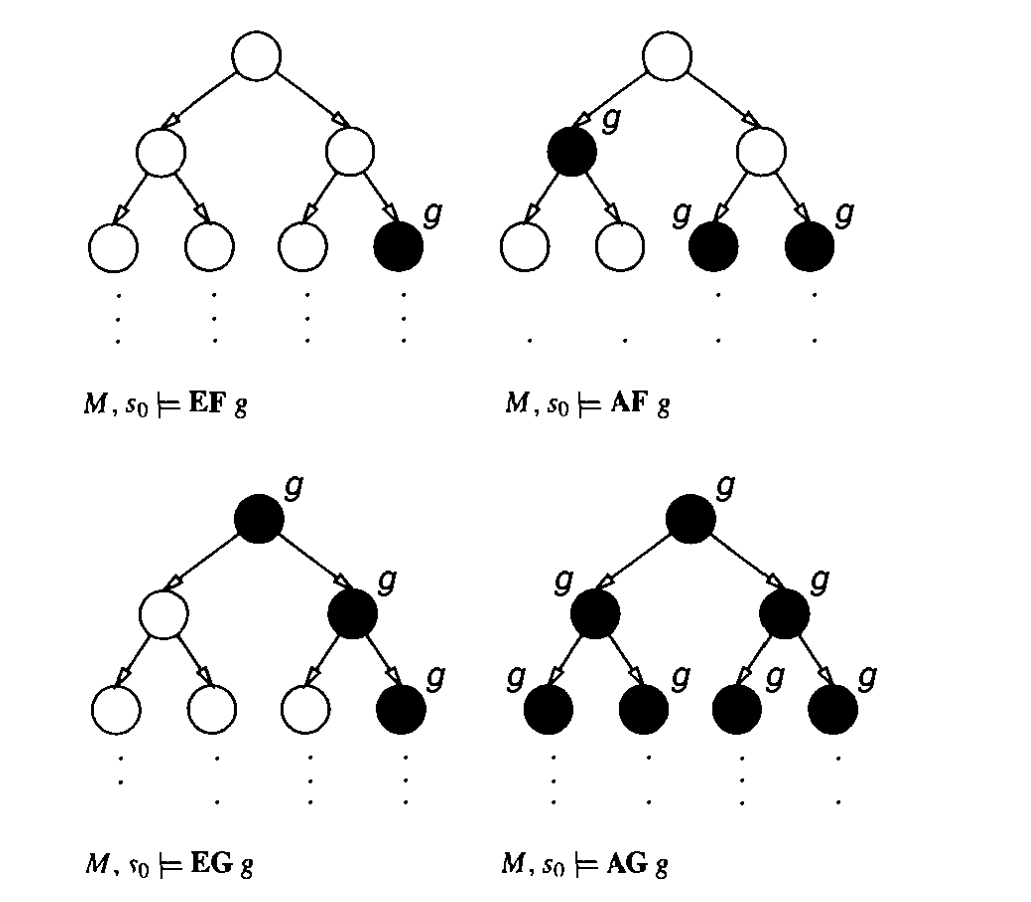
\includegraphics[width=\textwidth]{figure.png}
    \centering
    \caption{Βασικοί τελεστές της \english{CTL}}
    \label{fig:ops}
\end{figure}

Οι τέσσερις τελεστές που χρησιμοποιούνται περισσότερο φαίνονται στο Σχήμα \ref{fig:ops}.

Κάποι συνήθεις \english{CTL} τύποι που μπορεί να προκύψουν κατά την επαλήθευση ενός πεπερασμένου σύγχρονου προγράμματος είναι παρακάτω:

\begin{itemize}
    \item \english{$\mathbf{EF}(\text{Start} \wedge \neg \text{Ready})$}: Είναι δυνατόν να πάμε σε μια κατάσταση που το \english{Start} ισχύει, αλλά το \english{Ready} δεν ισχύει.
    \item \english{$\mathbf{AF}(\text{Req} \rightarrow \mathbf{AF} \text{Ack})$}: Αν υπάρξει κάποιο \english{Request}, τότε θα γίνει κάποια στιγμή \english{Aknowledge}
    \item \english{$\mathbf{AG}(\mathbf{AF} \text{DeviceEnabled})$}: Η πρόθεση \english{DeviceEnabled} ισχύει απείρως συχνά σε κάθε υπολογιστικό μονοπάτι.
    \item \english{$\mathbf{AG}(\mathbf{EF} \text{Restart})$}: Από κάθε κατάσταση είναι δυνατό να βρεθούμε στην κατάσταση \english{Restart} 
\end{itemize} 

\section*{Αλγόριθμος \english{Model Checking}}

Το πρόβλημα είναι: Δεδομένης μιας δομής \english{Kripke} $M = (S, R, L)$ που αναπαριστά ένα σύχρονο σύστημα πεπερασμένων καταστάσεων και ένα τύπο χρονικής λογικής $f$, ο οποίος περιγράφει κάποιο επιθυμητό \english{specification}, βρες το σύνολο όλων των καταστάσεων στο $S$ που ικανοποιούν το $f$:
\begin{equation*}
    {s \in S | M, s \models f}
\end{equation*}

Συνήθως, κάποιες καταστάσεις του συστήματος θεωρούνται αρχικές καταστάσεις. Το σύστημα ικανοποιεί το δωσμένο \english{specification} δεδομένου ότι όλες οι αρχικές καταστάσεις είναι στο σύνολο αυτό.

Ο αλγόριθμος θα λειτουργήσει αντιστοιχόντας σε κάθε κατάσταση $s$ το σύνολο \english{$\text{labels}(s)$} των υποτύπων του $f$ που είναι αληθείς στο $s$. Αρχικά το \english{$\text{labels}(s)$} είναι απλά $L(s)$. Ο αλγόριθμος περνάει από μια σειρά από βήματα. Κατά την διάρκεια του βήματος $i$, γίνετια επεξεργασία σε υποτύπους με $i - 1$ ενφωλιασμένους τελεστές. Όταν γίνει η επεξεργασία ενός υποτύπου, προστίθεται στην αντιστοίχηση της κάθε κατάστασης στην οποία είναι αληθής. Όταν ο αλγόρθμος τερματίσει, θα έχουμε ότι $M, s \models f$ ανν \english{$f \in \text{labels}(s)$}.

Όπως αναφέραμε και παραπάνω, υπάρχουν έξι περιπτώσεις που πρέπει να καλύπτει ο αλγόριθμός μας (και μια που είναι η περίπτωση της ατομικής πρότασης), αφού από αυτές τις έξι ($\neg f_1, f_1 \vee f_2, \mathbf{EX} f_1, \mathbf{E}[f_1 \mathbf{U} f_2], \mathbf{EG} f_1$ μπορούμε να καλύψουμε όλες τις υπόλοιπες.

\begin{itemize}
    \item Για τύπους που είναι ατομικές προτάσεις $f$, απλώς κάνουμε αντιστοίχηση όλες τις καταστάσεις για τις οποίες η $f$ είναι αληθής.
    \item Για τύπους της μορφής $\neg f_1$, κάνουμε αντιστοίχηση τις καταστάσεις που δεν αντιστοιχούν στην $f_1$.
    \item Για το $f_1 \vee f_2$, κάνουμε αντιστοίχηση κάθε κατάσταση που είναι αντιστοιχισμένη με την $f_1$ ή την $f_2$. 
    \item Για $\mathbf{EX} f_1$ κάνουμε αντιστοίχηση κάθε κατάσταση που έχει διάδοχο ο οποίος είναι αντιστοιχισμένος με την $f_1$.
    \item Για να διαχειριστούμε τύπους της μορφής $g = \mathbf{E}[f_1 \mathbf{U} f_2]$ θα βρούμε πρώτα όλες τις καταστάσεις που είναι αντιστοιχισμένες με την $f_2$. Μετά μετακινούμαστε προς τα πίσω χρησιμοποιώντας το αντίστροφο της σχέσης μετάβασης $R$ και βρίσκουμε όλες τις καταστάσεις που μπορούν να προσεγγιστούν από ένα μονοπάτι όπου κάθε κατάσταση είναι αντιστοιχισμένη με το $f_1$. Όλες αυτές οι καταστάσεις πρέπει να αντιστοιχηστούν με $g$.
    \item Για την περίπτωση $g = \mathbf{EG} f_1$, πρέπει να αποσυνθέσουμε τον γράφο σε μη-τετριμμένες ισχυρες συνδεδεμένες συνιστώσες. Μια ισχυρά συνδεδεμένη συνιστώσα $C$ είναι ένας μέγιστος υπογράφος, τέτοις ώστε κάθε κόμβος στον $C$ προσεγγίζεται από κάθε άλλον κόμβο στο $C$ κατά μήκος ενός κατευθυνόμενου μονοπατιού το οποίο περιέχεται εξ'ολοκλήρου μεσα στο $C$. Ο $C$ είναι μη-τετριμμένος ανν είτε έχει πάνω από ένα κόμβο ή περιέχει ένα κόμβο με αυτό-βρόχο. Έστω $M'$, το οποίο παίρνουμε από το $M$ διαγράφοντας από το $S$ όλες τις καταστάσεις στις οποίες ο $f_1$ δεν ισχύει και περιορίζοντας το $R$ και το $L$ αντίστοιχα. Έτσι $M' = (S', R', L')$ όπου $S' = {s \in S | M, s \models f_1}$, $R' = R|_{S' \times S'}$ και $L' = L|_{S'}$. Το $R'$ μπορεί να μην είναι ολικό σε αυτή την περίπτωση. Οι καταστάσεις που δεν έχουν εξερχόμενες μεταβάσεις μπορούν να διαγραφούν, αλλά αυτό δεν επηρεάζει την ορθότητα του αλγορίθμου. Ο αλγόριθμος βασίζεται στην παρατήρηση ότι: $M, s \models \mathbf{EG} f_1$ ανν ισχύουν οι παρακάτω δύο συνθήκες:
    \begin{enumerate}
        \item $s \in S'$
        \item Υπάρχει μονοπάτι στο $M'$ που οδηγεί από το $s$ σε κάποιο κόμβο $t$  σε μια μη-τετριμένη, ισχύρα συνδεδεμένη συνιστώσα $C$ του γράφου $(S', R')$.
    \end{enumerate}
    Με βάση αυτό και την δομή $M'$ που περιγράψαμε πριν, χωρίζουμε τον γράφο $(S', R')$ σε ισχυρά συνδεδεμένες συνιστώσες χρησιμοποιώντας τον αλγόριθμο του \english{Tarjan}. Μετά βρίσκουμε τις καταστάσεις που ανήκουν σε αυτές τις μη-τετριμμένες συνιστώσες. Έπειτα, δουλεύομε προς τα πίσω χρησιμοποιώντας το αντίστροφο της $R'$ και βρίσκουμε όλες τις καταστάσεις που μπορούν να προσεγγιστούν από ένα μονοπάτι όπου η κάθε κατάσταση είναι αντιστοιχισμένη με το $f_1$.
\end{itemize}

Για να διαχειριστούμε κάθε \english{CTL} τύπο $f$, εφαρμόζουμε διαδοχικά τον αλγόριθμο αντιστοίχησης στους υποτύπους του $f$, ξεκινώντας με το μικρότερο και πιο βαθεία εμφωλιασμένο και συνεχίζουμε προς τα έξω για να συμπεριλάβουμε όλο το $f$. Με αυτό τον τρόπο εγγυόμαστε ότι όποτε επεξεργαζόμαστε έναν υποτύπο του $f$, όλοι οι υποτύποι αυτού έχουν ήδη επεξεργαστεί. 

Θα παρουσιάσουμε τον αλγόριθμο σε ένα μικρό παράδειγμα που περιγράφει την λειτουργία του φούρνου μικροκυμάτων. Στο Σχήμα \ref{fig:microwave}, μπορούμε να δούμε την δομή \english{Kripke} για τον φούρνο. Για πληρότητα, σε κάθε κατάσταση φαίνονται οι ατομικές προτάσεις που ισχύουν σε αυτή, καθώς και οι αρνήσεις των προτάσεων που δεν είναι αληθής σε αυτή. Οι περιγραφές στις ακμές μας δείχνουν τις πράξεις που προκαλούν μεταβάσεις και δεν είναι μέρος της δομής.

\begin{figure}
    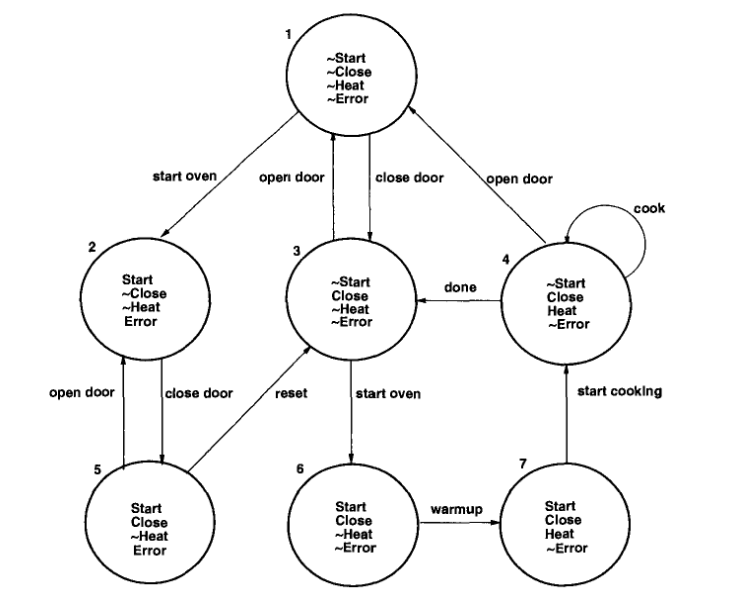
\includegraphics[width=\textwidth]{microwave.png}
    \centering
    \caption{Παράδειγμα φούρνου μικροκυμάτων}
    \label{fig:microwave}
\end{figure}


Ελέγχουμε τον τύπο \english{$\mathbf{AG} (\text{Start} \rightarrow \mathbf{AF} \text{Heat})$}, το οποίο είναι ισοδύναμο με την φόρμουλα \english{$\neg \mathbf{EF} (\text{Start} \wedge \mathbf{EG} \neg \text{Heat})$}. (Χρησιμοποιήσαμε το $\mathbf{EF} f$ ως συντομογραφία του \english{$\mathbf{E}[\text{true} \mathbf{U} f])$}. Ξεκινάμε υπολογίζοντας το σύνολο καταστάσεων που ικανοποιούν τους ατομικούς τύπους και συνεχίζουμε με πιο περίπλοκους τύπους. Έστω $S(g)$ το σύνολο όλων των καταστάσεων που αντιστοιχίζονται με τον ύποτυπο $g$. 
\begin{otherlanguage}{english}
    \begin{align*}
        S(\text{Start}) = {2, 5, 6, 7}\\
        S(\neg \text{Heat}) = {1, 2, 3, 5, 6}
    \end{align*}
\end{otherlanguage}

Για να υπολογίσουμε το \english{$S(\mathbf{EG} \neg \text{Heat})$} πρώτα βρίσκουμε το σύνολο των \\
μη-πεπερασμένων ισχυρά συνδεδεμένων συνιστοσών στο \english{$S' = S(\neg \text{Heat}) SCC = {{1,2,3,5}}$}. 
Συνεχίζουμε θέτοντας $T$, το σύνολο όλων των καταστάσεων που θα έπρεπε να αντιστοιχιστούν με το \english{$\mathbf{EG} \neg \text{Heat}$} να είναι η ένωση όλων των στοιχεών του $SCC$. 
Έτσι αρχικά $T={1,2,3,5}$. Καμία άλλη κατάσταση στο $S'$ δεν μπορεί να προσεγγίσει μια κατάσταση στο $T$ κατά μήκος ενός μονοπατιού στο $S'$. 
Άρα ο υπολογισμός τερματίζει με \english{$S(\mathbf{EG} \neg \text{Heat}) = {1,2,3,5}$}. 
Τέλος υπολογίζουμε το \english{$S(\text{Start} \wedge \mathbf{EG} \neg \text{Heat}) = {2, 5}$}. 

Όταν υπολογίζουμε το \english{$S(\mathbf{EF} (\text{Start} \wedge \mathbf{EG} \neg \text{Heat}))$}, ξεκινάμε θέτοντας \english{$T = S(\text{Start} \wedge \mathbf{EG} \neg \text{Heat})$}. Μετά χρησιμοποιούμε το αντίστροφο του πίνακα μεταβάσεων για να αντιστοιχίσουμε όλες τις καταστάσεις με τον τύπο στον οποίο αντιστοιχούν. Παίρνουμε:
\begin{otherlanguage}{english}
    \begin{equation*}
    S(\mathbf{EF}(\text{Start} \wedge \mathbf{EG} \neg \text{Heat})) = {1,2,3,4,5,6,7}
    \end{equation*}
\end{otherlanguage}

Έτσι υπολγίζουμε ότι \english{$S(\neg \mathbf{EF}(\text{Start} \wedge \mathbf{EG} \neg \text{Heat})) = 0$}. Αφού η αρχική κατάσταση δεν περιέχεται στο σύνολο, καταλήγουμε ότι το σύστημα δεν ικανοποιεί το \english{specification}.


\begin{otherlanguage}{english}
\printbibliography    
\end{otherlanguage}


\end{document}